\documentclass[a4paper]{article}

\usepackage[utf8]{inputenc}
\usepackage[portuguese]{babel}
\usepackage{a4wide}
\usepackage[pdftex]{hyperref}
\usepackage{graphicx}
\usepackage{wrapfig}
\usepackage{amsmath}
\usepackage{verbatim}
\usepackage{caption}
\usepackage{subcaption}
\usepackage{float}



\begin{document}

\begin{titlepage}
\begin{center}



\includegraphics[width=0.6\textwidth]{logo.jpg}\\[0.5cm]

{\large Universidade do Minho - Escola de Engenharia}\\[0.5cm]

{\large Relatório do trabalho prático de Sistemas Distribuidos}\\[0.5cm]

% Title
\rule{\linewidth}{0.5mm} \\[0.4cm]
{ \huge \bfseries Trabalho nº1 \\[0.4cm] }
\rule{\linewidth}{0.5mm} \\[1.5cm]

% Author and supervisor
\noindent
\begin{minipage}{0.4\textwidth}
  \begin{flushleft} \large
    \emph{Autores :}\\
    Daniel Maia \textsc{(A77531)}\\
    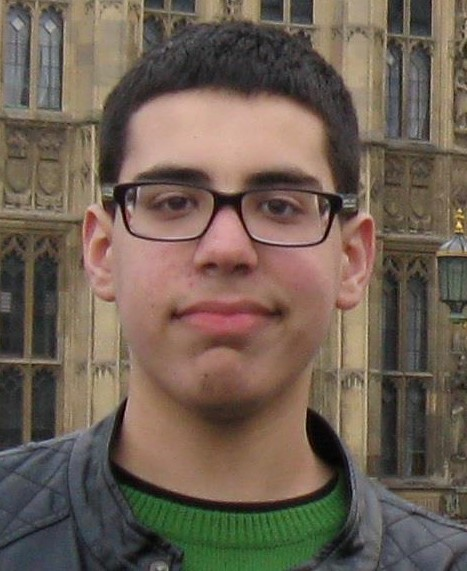
\includegraphics[width=1.5cm]{daniel.jpg}\break
    Diogo Silva\textsc{(A78034)}\\
    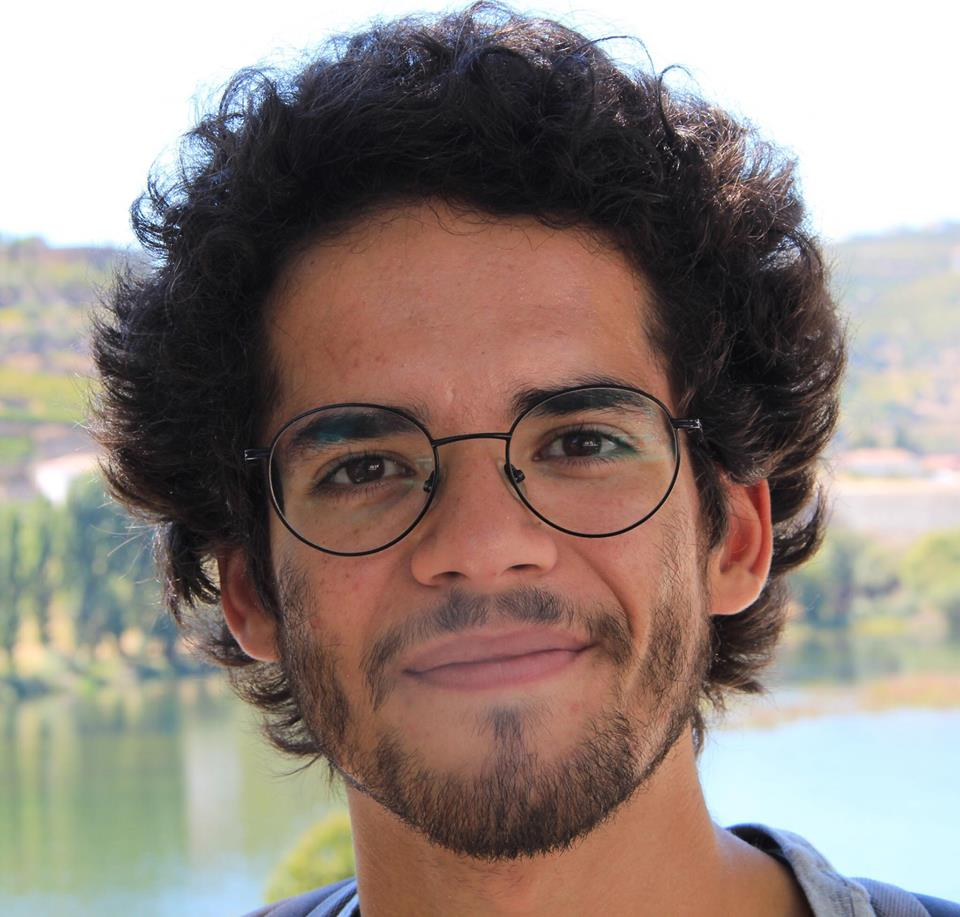
\includegraphics[width=1.5cm]{afonso.jpg}\break
    Marco Silva\textsc{(A79607)}\\
    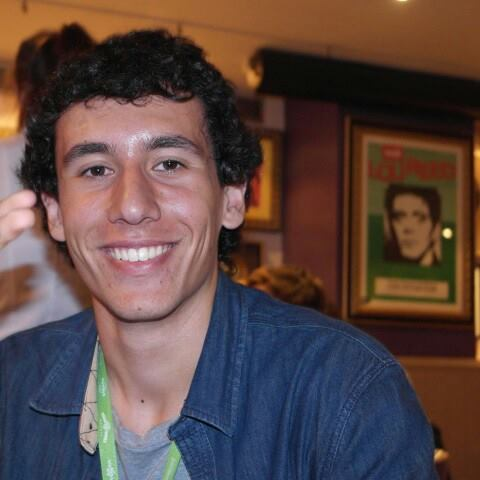
\includegraphics[width=1.5cm]{marco.jpg}\break
  \end{flushleft}
\end{minipage}%
\vfill

% Bottom of the page
{\large Versão 1.0 \\ \today}

\end{center}
\end{titlepage}




\begin{abstract}

\hspace{3mm} 

\end{abstract}

\pagebreak
\tableofcontents

\pagebreak
\section{Introdução}
\label{sec:1}

\hspace{3mm} 



%------------------------------------------------------------------------

\pagebreak
\section{Parte I}
\label{sec:2}

\hspace{3mm} 

\subsection{Rede do projeto}
\hspace{3mm} 

\pagebreak

\subsection{Matriz de incidência Vértice-Arco}
\hspace{3mm} Como segunda instância, era requerida a matriz de incidência associada ao grafo anterior (com \emph{n} vértices e \emph{m} arcos), com \emph{n} linhas e \emph{m} colunas. Cada coluna da matriz apresentada abaixo representa um arco do grafo, e a mesma está preenchida por -1, +1 e 0, que representam:


\begin{itemize}
    \item +1 na linha correspondente ao vértice de origem;
    \item -1 na linha correspondente ao vértice de destino;
    \item 0 nos restantes casos.
\end{itemize}


\par É de notar que se acrescentou, também, uma linha no fim da matriz, correspondente ao vetor dos custos dos arcos. Desta forma, segue-se a matriz de incidência Vértice-Arco para a rede em análise.




\subsection{Caminho crítico}
\hspace{3mm} 


%--------------------------------------------------------------------------

\pagebreak
\clearpage
\section{Parte II}
\label{sec:3}

\subsection{Apresentação do Modelo Alternativo de Progrmamação Linear}

\par 

\subsection{Matriz de incidência Vértice-Arco}

\par 

\pagebreak
\subsection{Input para o LPSolve}

\par 


%--------------------------------------------------------------------------

\pagebreak
\clearpage
\section{Parte III}
\label{sec:4}

\hspace{3mm}

\subsection{Rede do projeto}

\hspace{3mm} 

\subsection{Matriz de incidência Vértice-Arco}

\subsection{Input do programa Relax4}

\subsection{Output do programa Relax4}


\subsection{Interpretação do resultado}

\hspace{3mm} 


%------------------------------------------------------------------------
\pagebreak
\section{Conclusões}
\label{sec:5}

\hspace{3mm}  

\end{document}
